% !TeX spellcheck = en_GB
\documentclass[main.tex]{subfiles}

\begin{document}
\chapter{Data}
\lhead{Data}
\label{chap:data}

\section{Entity-annotated Danish Wikipedia}
\label{sec:dawiki}
For pretraining LUKE, a corpus of entity annotated text is needed.
Entity annotations consist of two things: The word span and the name of the entity.
No text is written directly with such annotations in mind.
However, some texts such as news articles often contain embedded hyperlinks that implicitly provide the word spans, but these often point to other articles rather than specific items.
On Wikipedia this is not the case, as hyperlinks point to articles on specific topics, which makes it useful for LUKE's pretraining task.
Given its size, Wikipedia then is a particularly useful pretraining dataset.

As of June 23rd, the Danish Wikipedia has 267,408 content pages containing a total of 81,822,460 words\footnote{\url{https://da.wikipedia.org/wiki/Speciel:Statistik}. Visited June 23, 2021.}.
The Danish Wikipedia from March 1st, 2021, which is marginally smaller, is used for building the dataset.
Yamada et al. limit the entity vocabulary to the 500,000 most often linked pages \cite{yamada2020luke}.
As the Danish Wikipedia is only roughly 2.5\pro\ the size of the English Wikipedia, no limit on the entity vocabulary is imposed to preserve data.

Every article is a sequence of words with embedded hyperlinks.
These are split into sequences of at most 512 tokens using BotXO's Danish BERT tokenizer, and the token spans of the hyperlinks are saved.
The first and last tokens are always [CLS] and [SEP], respectively, with the remaining 510 tokens coming directly from the tokenizer.
Sequences are cut short if necessary to prevent hyperlinks spanning two sequences.
All sequences contain text from at most one paragraph in an article.

Word spans over tokens is also saved, as the MLM pretraining task is done on a word level.
Sub-word and entity tokens are masked using the [MASK] token.
The [UNK] special token is reserved for sub-words that are not part of the tokenizer's vocabulary.

%TODO Make sure itemize is not broken up with a page
Thus, an entry in the dataset -- called an example -- consists of the following:
\begin{itemize}
    \item An array of at most 512 sub-words token ID's
    \item An array of at most 128 entity ID's
    \item An array of two-tuples containing the start and end indices for every entity
    \item An array of two-tuples containing the start and end indices for every word
\end{itemize}
The pretraining dataset is the set of all examples from all articles.

\subsection{Entity Augmentations}
\label{subsec:entaug}
For the purposes of the discussing the motivation and effects of our data preprocessing, we will use the terms true/false positive/negative about the entity annotations.
In order for the binary terms to make sense, annotations and no annotations are considered positive and negative, respectively, with only their existense being relevant.

One limitation of Wikipedia as a pretraining dataset is that hyperlinks are rarely repeated, even if the same article is refenced multiple times on a page.
This results in false negatives where entities are not annotated.

In order to augment the entity annotations, we perform preprocessing on Wikipedia prior to pretraining.
Our preprocessing consists of the following two steps applied article-wise:
\begin{enumerate}
    \item Get the set of mentioned articles including the title of the article itself.
    Only include titles of at least three characters.
    \item For each title, check if it matches a sequence of characters following a whitespace, ignoring casing.
    If there is a match, annotate and go to next whitespace.
\end{enumerate}
Many hyperlinks span only the first part of a given word.
For instance, this allows the words "Wind mills" to link to the article "Wind mill", even if they do not match exactly.
When matching, such matches are annotated as we expect it to remove a large number of false negatives, while introducing relatively few false positives.
To reduce the number of false positives, we only perform extra annotations with titles of at least three characters.
This prevents the article on "A" to be linked at every word starting with "A".
We also only match titles already linked in the articles, as we assume that any article that should be linked to has already been linked at least once.
This further reduces the number of false positives and whether this has positive effect on learning is subject to an experiment presented in Section~\ref{subsec:dataexp}.

Table \ref{tab:metadata} shows how these augmentation steps change the properties of the dataset.
\begin{table}[H]
    \centering
    \begin{tabular}{l|r|r|r}
        Statistic&Unaugmented	&Augmented    &Difference	\\\hline
        Subword tokens&101,394,208	&108,322,681 &+6,8\pro	\\
        Entity vocabulary size&214,150  &225,198    &+5,2\pro   \\
        Entity annotations&4,883,918	&7,180,372 &+47,0\pro\\
        Examples&363,498   &378,357 &+4,1\pro
    \end{tabular}
    \caption{
        Statistics for both datasets.
        The discrepancy in entity vocabulary size is explained by adding links that point to the article in which the link occurs.
        This means that some articles, which are never linked to, have links in the augmented dataset, leading to them being included in the entity vocabulary.
        The increased number of subword tokens and examples comes from not including sentences without entities, of which there are fewer in the augmented dataset.
    }
    \label{tab:metadata}
\end{table}\noindent


\section{Named Entity Recognition Benchmarks}
\label{sec:nerdata}

\subsection{Danish NER Test Sets}
\label{subsec:daNERdata}
For the task of benchmarking both existing and new Danish Named Entity Recognition (NER) models, three publicly available datasets previously used in the literature were identified.

\paragraph{Danish Universal Dependencies}
Danish Universal Dependencies of Danish Dependency Treebank (UD-DDT) is a grammatically annotated dataset produced by converting the Danish Dependency Treebank corpus \cite{kromann2003ddt} to the Universal Dependency annotation format \cite{johann2015udddt}.
The dataset consists of 5512 sentences and 100,733 tokens from the Danish PAROLE corpus containing book, newspaper and journal literature from 1983-1992 \cite{christensen1998parole}.
UD-DDT is split into training, development and test sets consisting of 4383, 564 and 565 sentences, respectively.
Two Named Entity Recognition (NER) annotations of this dataset are considered.
\begin{itemize}
    \item \emph{DaNE} is a 2020 NER annotation of the entire UD-DDT into four categories PER(son), ORG(anisation), LOC(ation), MISC(ellaneous) performed once by a linguist and once by non-linguists for the Alexandra Institute \cite[Sec. 4]{hvingelby2020dane}
    \item A NER annotation of the development and test subsets of UD-DDT into the same four entity categories was performed by Barbara Plank in 2019 \cite{plank2019neural}.
    A subset of the training data was also annotated.
    This annotation will be called \emph{Plank}.
\end{itemize}

\paragraph{Wikipedia Annotations}
Pan et al. performed an automatic NER annotation of a Wikipedia corpus in 2017 by transferring English NER of the categories PER, ORG, LOC to 281 languages including Danish \cite{pan2017wikiann}.
This dataset is known as \emph{Wiki-ANN} (Wikipedia Annotations) and the Danish version includes 40000 sentences.
Pan et al. consider this a "silver-standard" annotation due to its automatic generation which they label Knowledge Base mining \cite[1946]{pan2017wikiann}.
The balanced training, development and test splits from Rahimi et al. are used \cite{rahimi2019transfer}.

\paragraph{Summary}
The test sets of these three NER-annotated datasets were used and a summary of their counts is shown in Table~\ref{tab:daNERdata}.
DaNE is considered the main public Danish NER dataset, as it is produced with the highest degree of expert supervision and used for training most of the models compared in Section~\ref{sec:exidan}.
However, as shown on on Table \ref{tab:danedist} and Figure \ref{fig:dadatadist}, DaNE and Plank suffer from uneven label distributions in the different subsets.
As most model training assumes that the training data has the same distribution as the true distribution, this could cause evaluations on the test sets to give a poor view of real-world performance.
Previous literature has highlighted the scarcity of accessible, gold-standard, Danish NER as a limitation in the field \cite[Sec. 2.1]{plank2019neural}.
\begin{table}[H]
    \centering
    \begin{tabular}{l|rrr|rrrr}
        \multirow{2}{*}{Dataset} & \multicolumn{3}{c|}{Number of sentences} & \multicolumn{4}{c}{Test set entities}\\
                                &\jl{Train} & \jl{Dev.} & \jl{Test} &\multicolumn{1}{|l}{LOC} & \jl{PER} & \jl{ORG} & \jl{MISC} \\\hline
        DaNE        & 4,383 & 564 & 565 & 101 & 318 & 221 & 159 \\
        Plank       & 604  & 564 & 565 & 98  & 309 & 114 & 52 \\
        Wiki-ANN (da.)   & $20\ctp3$ & $10\ctp3$ & $10\ctp3$ & 7,458 & 10,660 & 10,876 & 0
    \end{tabular}
    \caption{
        Counts of sentences and test set entities in the three Danish NER benchmarks.
        Note the clear differences in annotations between DaNE and Plank, which use the same text corpus.
    }
    \label{tab:daNERdata}
\end{table}

\begin{table}[H]
    \centering
    \begin{tabular}{l|r r r r}
        Subset of data&LOC	&PER	&ORG   &MISC \\\hline
        Train&1,144	&2,146	&1,267  &1,273 \\
        Dev.&126	&277   &131  &138 \\
        Test&101   &318   &221  &159
    \end{tabular}
    \caption{DaNE label distribution by data subset.}
    \label{tab:danedist}
\end{table}\noindent

\begin{figure}[H]
    \centering
   	\begin{minipage}[t]{0.32\textwidth}
       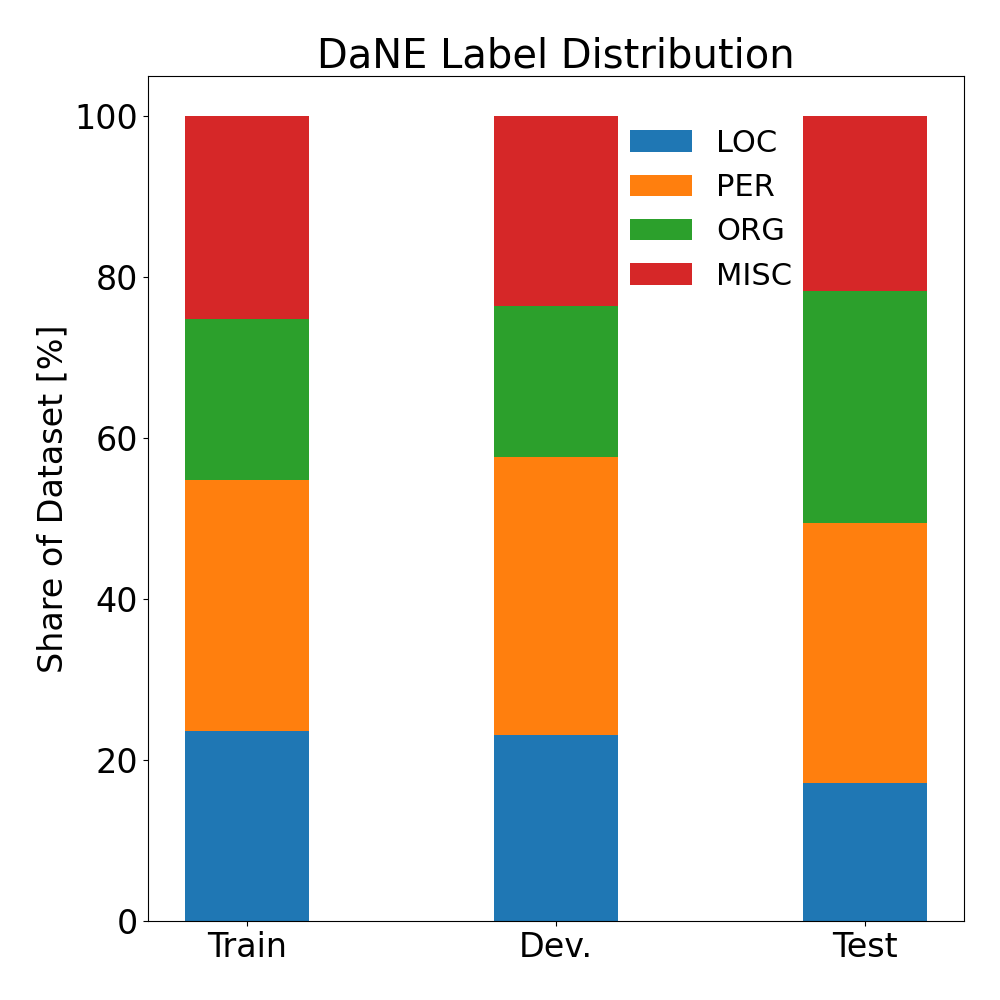
\includegraphics[width=\textwidth]{datadist_dane}
    \end{minipage}\hfill
    \begin{minipage}[t]{0.32\textwidth}
        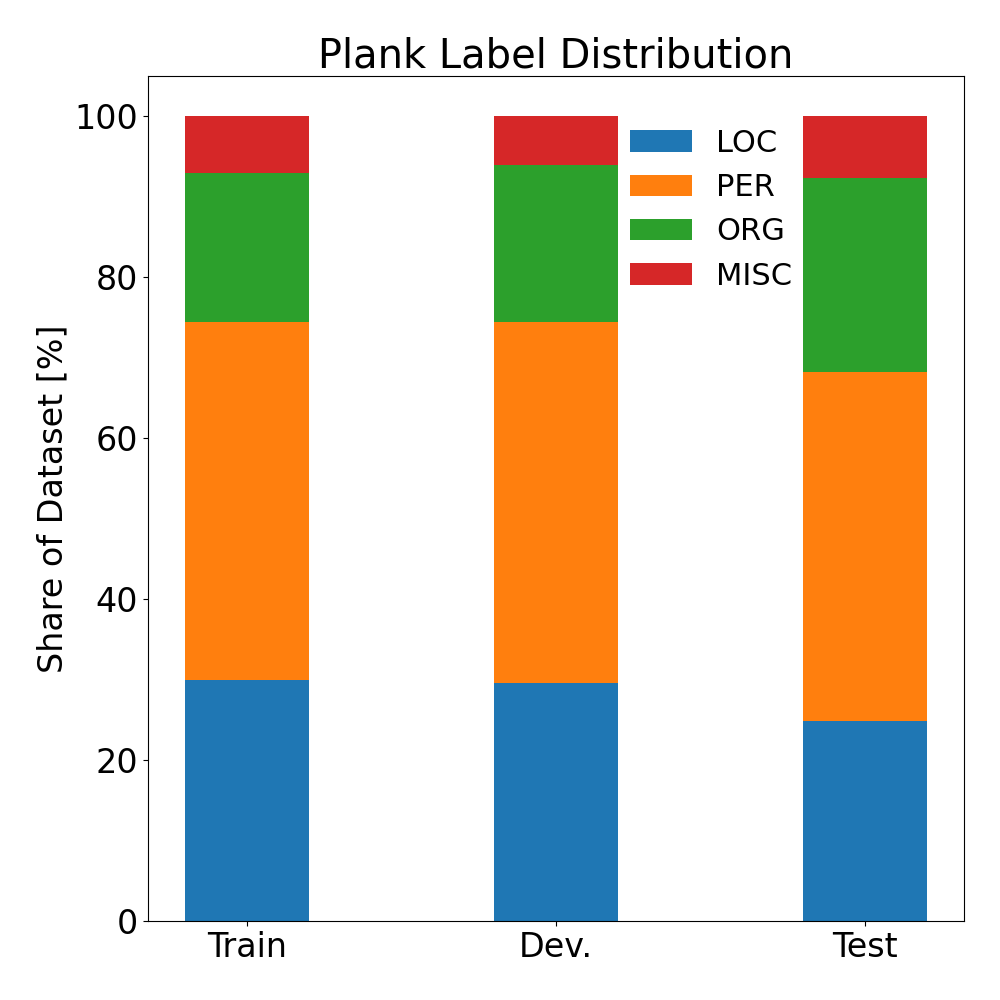
\includegraphics[width=\textwidth]{datadist_plank}
    \end{minipage}\hfill
    \begin{minipage}[t]{0.32\textwidth}
        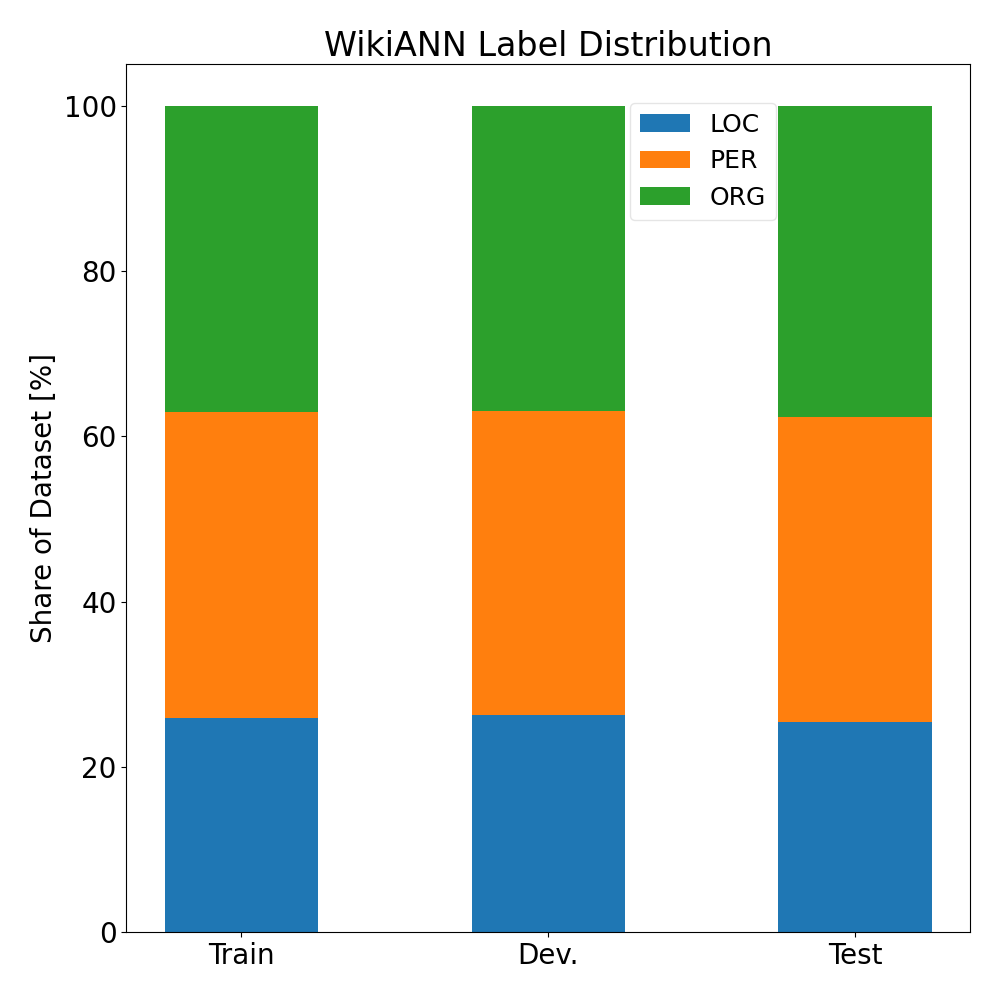
\includegraphics[width=\textwidth]{datadist_wikiann}
    \end{minipage}
    \caption{Distribution of entity labels in the three Danish NER datasets.}
    \label{fig:dadatadist}
\end{figure}\noindent

\subsection{CoNLL-2003}
The shared task for the 2003 Conference on Computational Natural Language Leanring (CoNLL) was language-independent NER for which annotations on English Reuters news wire articles were performed by researchers \cite{tjang2003conll}.
This corpus consists of 1393 articles that were divided into training, development and test sets as seen in Table~\ref{tab:conll2003}.
The dataset is the central benchmark in the field of Named Entity Recognition \cite[Sec. 4.3]{yamada2020luke} and has a competitive history with over 50 models submitted to the performance leaderboard at Papers With Code\footnotemark.
\footnotetext{
    See 
    \url{
        https://paperswithcode.com/sota/named-entity-recognition-ner-on-conll-2003
    }.
    As of February 2, 2021, LUKE tops the leaderboard.
}
\begin{table}[H]
    \centering
    \begin{tabular}{l|rrr|rrrr}
    CoNLL-2003 English  & Articles  & Sentences  & Tokens   & LOC   & PER   & ORG   & MISC  \\ \hline
    Training set        & 946       & 14,987     & 203,621  & 7140  & 6600  & 6321  & 3438   \\
    Development set     & 216       & 3466      & 51,362   & 1837  & 1842  & 1341  & 922    \\
    Test set            & 231       & 3684      & 46,435   & 1668  & 1617  & 1661  & 702    \\
    \end{tabular}
    \caption{
        Dataset counts for the canonical NER dataset CoNLL-2003.
        Note the more even distribution of entities when compared to the Danish NER datasets shown at Table~\ref{tab:daNERdata}, highlighting the difference in entities between short news texts and more general-purpose literature.
    }
    \label{tab:conll2003}
\end{table}

\subsection{Annotation Schemes: What Do The Tags Mean?}
\label{subsec:annoschemes}
The DaNE and Plank sets refer to the CoNLL-2003 as their reference annotation scheme \cite[Sec. 4]{hvingelby2020dane} \cite[Sec. 2.1]{plank2019neural}.
Wiki-ANN follows the same categories, excluding MISC.
All datasets follow the Inside-outside-beginning (IOB) format that ascribes a word the "I-X" tag if it is inside a named entity of type X, "B-X" if it begins the X entity and "O" if it is outside named entities (e.g. the null class).
This format proposed by Ramshaw and Marcus in 1995 is widely used but does allow entities to be nested or to overlap \cite{ramshaw1995IOB}.

The definition of the annotation categories are given in the CoNLL-2003 guidelines \footnotemark and are summarized here:
\footnotetext{
    These are available here: \url{https://www.clips.uantwerpen.be/conll2003/ner/annotation.txt} (collected 27/02-2021)
}
\begin{itemize}
    \item LOC: Geographical regions, natural locations and public and commercial places. Also includes abstract places.
    \item PER: Names, aliases of people, animals and fictional characters.
    \item ORG: Companies, brands, government bodies, movements, clubs and subdivisions thereof.
    \item MISC: Titles of media, nationalities, languages, religions, ideologies, wars, slogans, eras, but also both adjectives and word combinations that are derived from one of the other tags.
\end{itemize}
To end the introduction of the data, some examples of named entities in each testing dataset are shown.
Note, that the all-important context of the words is not shown here.
\begin{itemize}
    \item DaNE: helvede (LOC), Holland (LOC), Astrid Lindgren (PER), Odense Teater (ORG), det danske rigsfællesskab (ORG), afghansk (MISC), Camel (MISC)
    \item Plank: Bagdad (LOC), Bjarne (PER), USA (ORG), Københavns Kommune (ORG), DR-dokumentar (MISC), Levi's jeans (MISC)
    \item Wiki-ANN (da.): Dinariske Alper (LOC), Esbjerg Kommune (LOC), Jorge Luis Borges (PER), FC Barcelona (ORG), kommunehospitals (ORG)
    \item CoNLL-2003: Buenos Aires (LOC), Whistler Mountain (LOC), Katja Seizinger (PER),  FIFA (ORG), Asian Cup (MISC), Swede (MISC)
\end{itemize}

\end{document}
